\documentclass{standalone}
\usepackage{tikz}

% Color Definitions
\definecolor{SourceColor}{RGB}{85,168,104}
\definecolor{TargetColor}{RGB}{221,132,82}
\definecolor{AbsorbingAreaColor}{RGB}{196,78,82}
\definecolor{ObstacleColor}{RGB}{179,179,179}
\definecolor{StairColor}{RGB}{129,114,178}
\definecolor{AgentColor}{RGB}{0,0,255}

% Draw Settings
\newcommand{\AgentRadius}{0.195000}
\newcommand{\LineWidth}{1}

\begin{document}
% Change scaling to [x=1mm,y=1mm] if TeX reports "Dimension too large".
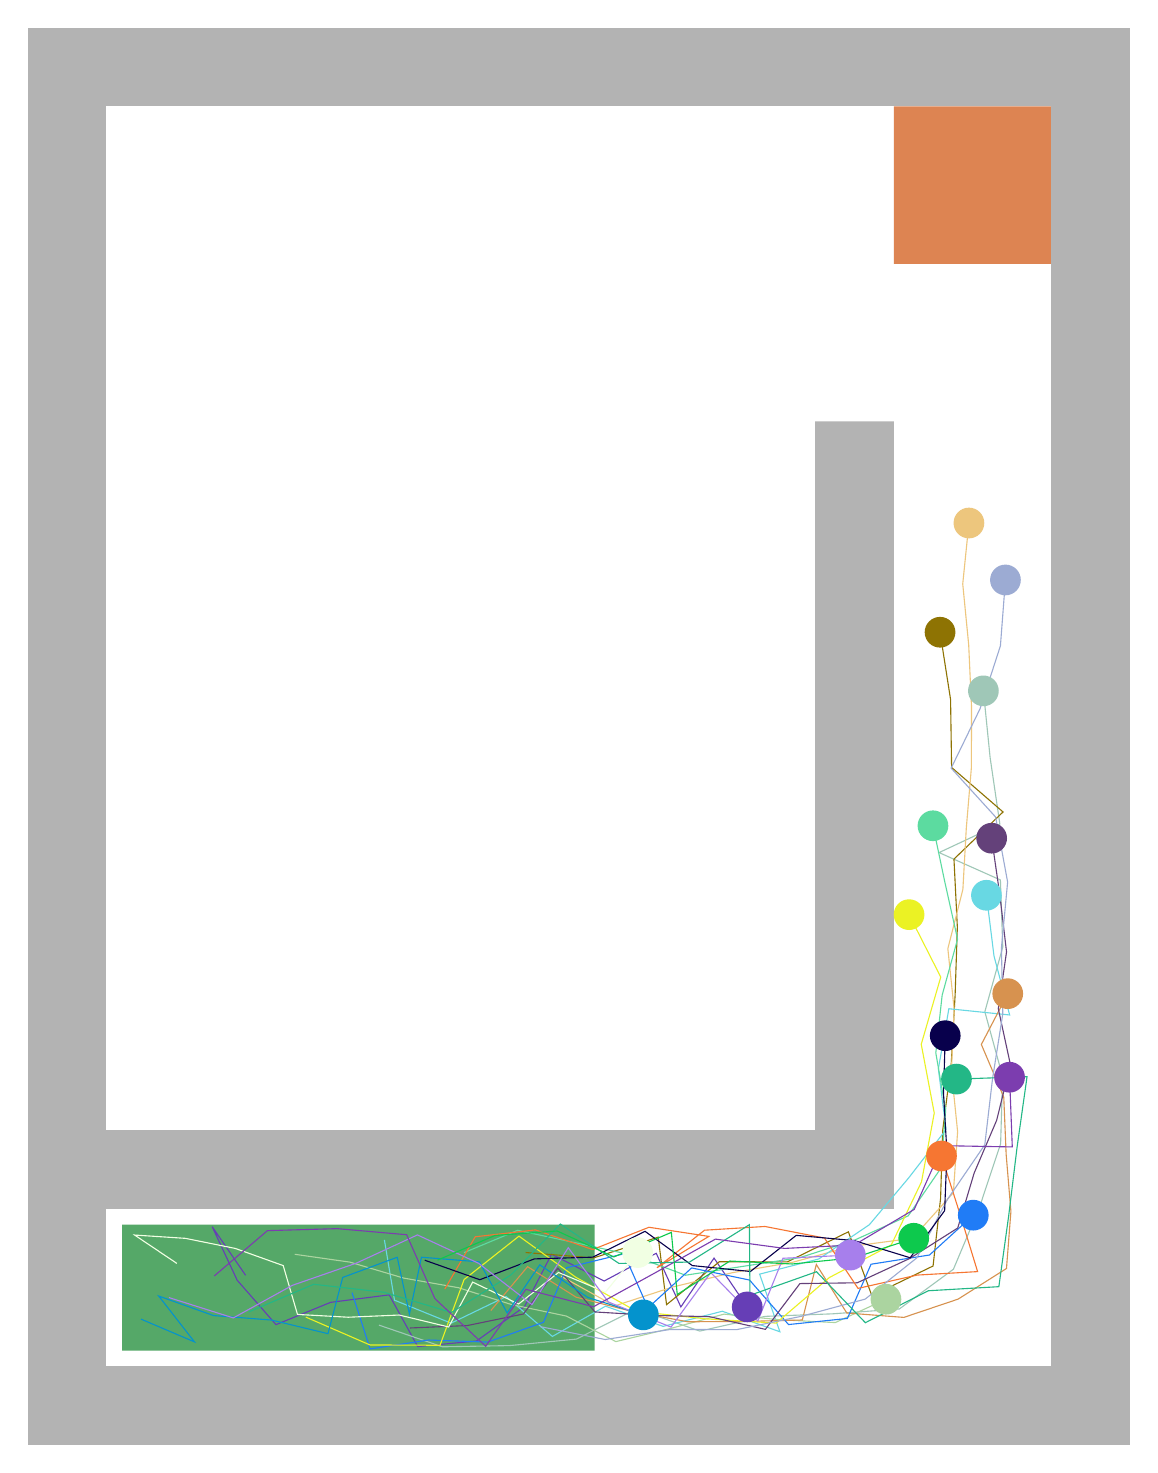
\begin{tikzpicture}[x=1cm,y=1cm]
% Clipping
\clip (0.000000,0.000000) rectangle (14.000000,18.000000);
% Ground
\fill[white] (0.000000,0.000000) rectangle (14.000000,18.000000);
% Sources
\fill[SourceColor] (1.200000,1.200000) to (7.200000,1.200000) to (7.200000,2.800000) to (1.200000,2.800000) to (1.200000,1.200000);
% Targets
\fill[TargetColor] (11.000000,15.000000) to (13.000000,15.000000) to (13.000000,17.000000) to (11.000000,17.000000) to (11.000000,15.000000);
% Absorbing Areas
% Obstacles
\draw[ObstacleColor,line width=1cm] (0.500000,0.500000) rectangle (13.500000,17.500000);
\fill[ObstacleColor] (0.800000,3.000000) to (11.000000,3.000000) to (11.000000,4.000000) to (0.800000,4.000000) to (0.800000,3.000000);
\fill[ObstacleColor] (10.000000,4.000000) to (11.000000,4.000000) to (11.000000,13.000000) to (10.000000,13.000000) to (10.000000,4.000000);
% Stairs
% Trajectories
% Trajectory Agent 1 @ step (28, null) of (62, null)
\draw[draw={rgb,255: red,102; green,62; blue,182}]
(9.138079,1.753357) to
(8.716766,2.373529) to
(8.716766,2.373529) to
(8.295360,1.753419) to
(7.982511,2.434774) to
(7.982511,2.434774) to
(7.982511,2.434774) to
(7.982511,2.434774) to
(7.982511,2.434774) to
(7.320749,2.082369) to
(6.653149,2.423587) to
(6.653149,2.423587) to
(6.653149,2.423587) to
(6.309488,1.757242) to
(6.309488,1.757242) to
(5.699807,1.320884) to
(4.953425,1.249942) to
(4.953425,1.249942) to
(4.591471,1.906530) to
(4.591471,1.906530) to
(4.591471,1.906530) to
(3.847736,1.811788) to
(3.153585,1.528461) to
(3.153585,1.528461) to
(2.660458,2.093213) to
(2.343254,2.772551) to
(2.343254,2.772551) to
(2.767963,2.154699);
% Trajectory Agent 2 @ step (28, null) of (37, null)
\draw[draw={rgb,255: red,159; green,199; blue,183}]
(12.137592,9.577429) to
(12.223067,8.729046) to
(12.223067,8.729046) to
(12.346888,7.885405) to
(11.574786,7.523580) to
(12.353372,7.175927) to
(12.383710,6.323788) to
(12.383710,6.323788) to
(12.155895,5.502107) to
(12.381567,4.679834) to
(12.356362,3.827528) to
(12.087844,3.018233) to
(12.087844,3.018233) to
(11.756917,2.232391) to
(11.069809,1.727473) to
(10.219377,1.665624) to
(9.367299,1.633619) to
(9.367299,1.633619) to
(8.535393,1.446554) to
(7.730461,1.727881) to
(7.730461,1.727881) to
(6.968596,1.344968) to
(6.968596,1.344968) to
(6.968596,1.344968) to
(6.119928,1.262366) to
(5.267388,1.247030) to
(5.267388,1.247030) to
(4.460515,1.522739);
% Trajectory Agent 3 @ step (28, null) of (36, null)
\draw[draw={rgb,255: red,142; green,115; blue,3}]
(11.586981,10.321767) to
(11.586981,10.321767) to
(11.720664,9.468282) to
(11.733752,8.604491) to
(12.387098,8.039294) to
(12.387098,8.039294) to
(11.763811,7.441113) to
(11.806731,6.578289) to
(11.806731,6.578289) to
(11.778479,5.714860) to
(11.729878,4.852338) to
(11.729878,4.852338) to
(11.620760,3.995366) to
(11.593880,3.131893) to
(11.593880,3.131893) to
(11.498503,2.273284) to
(10.721173,1.896370) to
(10.721173,1.896370) to
(10.422896,2.707134) to
(9.647731,2.325786) to
(9.647731,2.325786) to
(8.783842,2.327289) to
(8.113642,1.782184) to
(8.113642,1.782184) to
(8.007983,2.639589) to
(7.185443,2.375512) to
(7.185443,2.375512) to
(6.324299,2.444339);
% Trajectory Agent 4 @ step (28, null) of (35, null)
\draw[draw={rgb,255: red,237; green,198; blue,125}]
(11.953786,11.708995) to
(11.953786,11.708995) to
(11.875186,10.935508) to
(11.950817,10.161724) to
(11.950817,10.161724) to
(11.986214,9.385060) to
(11.985390,8.607589) to
(11.985390,8.607589) to
(11.920388,7.832841) to
(11.877098,7.056576) to
(11.686133,6.302923) to
(11.686133,6.302923) to
(11.766484,5.529615) to
(11.731162,4.752947) to
(11.731162,4.752947) to
(11.810078,3.979492) to
(11.756024,3.203903) to
(11.756024,3.203903) to
(11.236781,2.625243) to
(10.466031,2.523236) to
(10.466031,2.523236) to
(9.715404,2.320702) to
(8.949311,2.188176) to
(8.949311,2.188176) to
(8.193278,2.006865) to
(7.454076,1.765947) to
(7.454076,1.765947) to
(6.774616,2.143830);
% Trajectory Agent 5 @ step (28, null) of (42, null)
\draw[draw={rgb,255: red,104; green,216; blue,227}]
(12.176111,6.981362) to
(12.272024,6.211267) to
(12.470925,5.461143) to
(11.698929,5.540319) to
(11.698929,5.540319) to
(11.565656,4.775803) to
(11.663544,4.005956) to
(11.188642,3.392185) to
(11.188642,3.392185) to
(10.689629,2.797852) to
(10.047212,2.362482) to
(9.295451,2.169862) to
(9.553200,1.437871) to
(9.553200,1.437871) to
(8.822235,1.698518) to
(8.070403,1.506178) to
(7.337980,1.762697) to
(7.337980,1.762697) to
(6.663728,1.378469) to
(6.076027,1.885277) to
(5.377416,1.547359) to
(5.377416,1.547359) to
(5.377416,1.547359) to
(4.658388,1.839328) to
(4.530264,2.604724) to
(4.530264,2.604724) to
(4.530264,2.604724) to
(4.530264,2.604724);
% Trajectory Agent 6 @ step (28, null) of (68, null)
\draw[draw={rgb,255: red,171; green,212; blue,160}]
(10.900026,1.851337) to
(10.900026,1.851337) to
(10.256417,1.554671) to
(9.548632,1.590495) to
(9.548632,1.590495) to
(8.843542,1.661849) to
(8.843542,1.661849) to
(8.843542,1.661849) to
(8.843542,1.661849) to
(8.159006,1.478399) to
(8.159006,1.478399) to
(7.469858,1.313115) to
(7.469858,1.313115) to
(6.839867,1.637698) to
(6.839867,1.637698) to
(6.146263,1.783151) to
(6.146263,1.783151) to
(6.146263,1.783151) to
(6.146263,1.783151) to
(5.470754,1.997467) to
(5.470754,1.997467) to
(4.772777,2.120229) to
(4.772777,2.120229) to
(4.093451,2.322118) to
(4.093451,2.322118) to
(3.391834,2.422008) to
(3.391834,2.422008) to
(3.391834,2.422008);
% Trajectory Agent 7 @ step (28, null) of (51, null)
\draw[draw={rgb,255: red,215; green,146; blue,79}]
(12.446823,5.731792) to
(12.446823,5.731792) to
(12.111532,5.086604) to
(12.396204,4.417537) to
(12.396204,4.417537) to
(12.426545,3.691060) to
(12.426545,3.691060) to
(12.487026,2.966470) to
(12.430814,2.241536) to
(12.430814,2.241536) to
(11.816424,1.852673) to
(11.816424,1.852673) to
(11.127409,1.620409) to
(10.402474,1.676606) to
(10.402474,1.676606) to
(10.015737,2.292336) to
(10.015737,2.292336) to
(9.837675,1.587366) to
(9.110796,1.569049) to
(9.110796,1.569049) to
(8.383697,1.565027) to
(8.383697,1.565027) to
(7.668749,1.697457) to
(6.964323,1.877657) to
(6.964323,1.877657) to
(6.348783,2.264696) to
(6.348783,2.264696) to
(5.881952,1.707240);
% Trajectory Agent 8 @ step (28, null) of (46, null)
\draw[draw={rgb,255: red,92; green,219; blue,160}]
(11.497106,7.864177) to
(11.497106,7.864177) to
(11.649177,7.142938) to
(11.809591,6.423508) to
(11.809591,6.423508) to
(11.613857,5.712875) to
(11.613857,5.712875) to
(11.533043,4.980223) to
(11.658409,4.253866) to
(11.658409,4.253866) to
(11.600550,3.519044) to
(11.600550,3.519044) to
(11.183638,2.911182) to
(10.512267,2.606927) to
(10.512267,2.606927) to
(10.512267,2.606927) to
(10.512267,2.606927) to
(9.810799,2.380531) to
(9.082286,2.268373) to
(9.082286,2.268373) to
(8.353817,2.155931) to
(8.353817,2.155931) to
(7.663740,2.414977) to
(6.943384,2.571179) to
(6.943384,2.571179) to
(6.222887,2.726725) to
(6.222887,2.726725) to
(5.542507,2.443186);
% Trajectory Agent 9 @ step (28, null) of (56, null)
\draw[draw={rgb,255: red,32; green,124; blue,246}]
(12.009078,2.918682) to
(12.009078,2.918682) to
(11.453231,2.412933) to
(10.710915,2.295823) to
(10.710915,2.295823) to
(10.410535,1.606969) to
(9.663025,1.529662) to
(9.663025,1.529662) to
(9.663025,1.529662) to
(9.167615,2.094743) to
(8.432060,2.248715) to
(8.432060,2.248715) to
(7.877677,1.741362) to
(7.573546,2.428568) to
(7.573546,2.428568) to
(7.573546,2.428568) to
(6.843392,2.250740) to
(6.843392,2.250740) to
(6.843392,2.250740) to
(6.550634,1.558612) to
(6.550634,1.558612) to
(6.550634,1.558612) to
(5.842608,1.306728) to
(5.842608,1.306728) to
(5.091579,1.333269) to
(4.348686,1.219878) to
(4.348686,1.219878) to
(4.119342,1.935523);
% Trajectory Agent 10 @ step (28, null) of (44, null)
\draw[draw={rgb,255: red,235; green,242; blue,36}]
(11.193520,6.735295) to
(11.193520,6.735295) to
(11.596060,5.942835) to
(11.348184,5.089260) to
(11.348184,5.089260) to
(11.513465,4.215925) to
(11.351614,3.341947) to
(10.967370,2.540456) to
(10.967370,2.540456) to
(10.180815,2.126495) to
(9.505994,1.548008) to
(9.505994,1.548008) to
(8.618761,1.601398) to
(8.618761,1.601398) to
(7.735018,1.696419) to
(6.959887,2.131396) to
(6.239726,2.652356) to
(6.239726,2.652356) to
(5.542379,2.101232) to
(5.236506,1.266682) to
(4.347676,1.270393) to
(4.347676,1.270393) to
(4.347676,1.270393) to
(4.347676,1.270393) to
(3.532376,1.624394) to
(3.532376,1.624394) to
(3.532376,1.624394) to
(3.532376,1.624394);
% Trajectory Agent 11 @ step (28, null) of (42, null)
\draw[draw={rgb,255: red,100; green,65; blue,122}]
(12.242398,7.706203) to
(12.242398,7.706203) to
(12.346185,6.985398) to
(12.431441,6.262166) to
(12.326623,5.541509) to
(12.326623,5.541509) to
(12.480889,4.829797) to
(12.305663,4.122953) to
(12.019953,3.453100) to
(11.811634,2.755292) to
(11.811634,2.755292) to
(11.196192,2.365982) to
(10.535370,2.059963) to
(9.807198,2.050016) to
(9.807198,2.050016) to
(9.368777,1.468536) to
(8.658678,1.630065) to
(7.930609,1.645830) to
(7.930609,1.645830) to
(7.203686,1.689592) to
(7.203686,1.689592) to
(6.733500,2.245701) to
(6.733500,2.245701) to
(6.295662,1.663781) to
(6.295662,1.663781) to
(5.582433,1.516688) to
(5.582433,1.516688) to
(4.854846,1.485860);
% Trajectory Agent 12 @ step (28, null) of (77, null)
\draw[draw={rgb,255: red,241; green,255; blue,227}]
(7.746160,2.443621) to
(7.746160,2.443621) to
(7.746160,2.443621) to
(7.746160,2.443621) to
(7.338273,1.942236) to
(6.741825,2.191254) to
(6.741825,2.191254) to
(6.234794,1.790407) to
(6.234794,1.790407) to
(5.651333,2.068496) to
(5.651333,2.068496) to
(5.346084,1.498774) to
(4.717808,1.650525) to
(4.717808,1.650525) to
(4.072068,1.622593) to
(4.072068,1.622593) to
(3.426700,1.658078) to
(3.426700,1.658078) to
(3.245190,2.278412) to
(3.245190,2.278412) to
(3.245190,2.278412) to
(2.636692,2.496332) to
(2.636692,2.496332) to
(2.003165,2.624407) to
(2.003165,2.624407) to
(1.358183,2.666346) to
(1.358183,2.666346) to
(1.894731,2.305961);
% Trajectory Agent 13 @ step (28, null) of (55, null)
\draw[draw={rgb,255: red,246; green,118; blue,50}]
(11.605332,3.670113) to
(11.605332,3.670113) to
(11.838877,2.937395) to
(12.063789,2.201981) to
(12.063789,2.201981) to
(11.296016,2.157903) to
(10.545758,1.988988) to
(10.545758,1.988988) to
(10.118668,2.628528) to
(9.363737,2.775153) to
(9.363737,2.775153) to
(9.363737,2.775153) to
(8.596158,2.727827) to
(8.596158,2.727827) to
(8.596158,2.727827) to
(7.992404,2.251486) to
(8.650661,2.649125) to
(8.650661,2.649125) to
(7.890417,2.765093) to
(7.175333,2.482122) to
(7.175333,2.482122) to
(6.447845,2.731481) to
(5.683783,2.644146) to
(5.683783,2.644146) to
(5.683783,2.644146) to
(5.683783,2.644146) to
(5.683783,2.644146) to
(5.297056,1.979419);
% Trajectory Agent 14 @ step (28, null) of (35, null)
\draw[draw={rgb,255: red,156; green,171; blue,211}]
(12.417572,10.985764) to
(12.417572,10.985764) to
(12.353697,10.148928) to
(12.095112,9.350486) to
(12.095112,9.350486) to
(11.728148,8.595692) to
(12.293000,7.974953) to
(12.445292,7.149615) to
(12.445292,7.149615) to
(12.366713,6.314031) to
(12.383789,5.474934) to
(12.383789,5.474934) to
(12.252793,4.645949) to
(12.155184,3.812374) to
(12.155184,3.812374) to
(11.681419,3.119610) to
(11.292027,2.376139) to
(11.292027,2.376139) to
(10.636099,1.852560) to
(10.636099,1.852560) to
(10.636099,1.852560) to
(9.825663,1.634458) to
(9.003686,1.464964) to
(9.003686,1.464964) to
(8.164418,1.467404) to
(7.334956,1.339471) to
(7.334956,1.339471) to
(6.511704,1.502667);
% Trajectory Agent 15 @ step (28, null) of (53, null)
\draw[draw={rgb,255: red,8; green,0; blue,76}]
(11.652883,5.198204) to
(11.652883,5.198204) to
(11.631404,4.457167) to
(11.631404,4.457167) to
(11.674632,3.717080) to
(11.674632,3.717080) to
(11.645549,2.976303) to
(11.645549,2.976303) to
(11.645549,2.976303) to
(11.208026,2.377829) to
(11.208026,2.377829) to
(10.499336,2.595444) to
(10.499336,2.595444) to
(9.761011,2.662323) to
(9.178666,2.203551) to
(9.178666,2.203551) to
(9.178666,2.203551) to
(9.178666,2.203551) to
(8.441114,2.278478) to
(8.441114,2.278478) to
(7.840746,2.713398) to
(7.175869,2.385470) to
(7.175869,2.385470) to
(6.434848,2.363443) to
(6.434848,2.363443) to
(5.742273,2.098989) to
(5.742273,2.098989) to
(5.043423,2.346388);
% Trajectory Agent 16 @ step (28, null) of (63, null)
\draw[draw={rgb,255: red,4; green,147; blue,205}]
(7.819136,1.652575) to
(7.819136,1.652575) to
(7.114579,1.873333) to
(6.503675,2.287976) to
(6.503675,2.287976) to
(6.089394,1.676826) to
(5.737206,2.325745) to
(5.737206,2.325745) to
(5.001227,2.384638) to
(4.848188,1.662341) to
(4.848188,1.662341) to
(4.693278,2.384239) to
(4.693278,2.384239) to
(4.693278,2.384239) to
(4.693278,2.384239) to
(4.693278,2.384239) to
(4.000828,2.128023) to
(4.000828,2.128023) to
(3.813507,1.413850) to
(3.095748,1.586928) to
(3.095748,1.586928) to
(2.359599,1.643657) to
(2.359599,1.643657) to
(2.359599,1.643657) to
(1.664311,1.892067) to
(2.118100,1.309651) to
(2.118100,1.309651) to
(1.438766,1.598856);
% Trajectory Agent 17 @ step (28, null) of (45, null)
\draw[draw={rgb,255: red,35; green,183; blue,134}]
(11.795608,4.646983) to
(12.691871,4.676916) to
(12.691871,4.676916) to
(12.566156,3.789009) to
(12.457271,2.898882) to
(12.457271,2.898882) to
(12.333846,2.010654) to
(12.333846,2.010654) to
(11.438579,1.958887) to
(10.638814,1.553229) to
(10.638814,1.553229) to
(10.018142,2.200491) to
(10.018142,2.200491) to
(9.172841,1.901077) to
(9.165954,2.797813) to
(9.165954,2.797813) to
(8.405120,2.323140) to
(8.405120,2.323140) to
(7.508522,2.305998) to
(6.764352,2.806390) to
(6.140394,2.162295) to
(6.140394,2.162295) to
(6.140394,2.162295) to
(5.382610,1.682768) to
(4.523569,1.940122) to
(3.632497,2.040991) to
(3.632497,2.040991) to
(2.807389,1.689738);
% Trajectory Agent 18 @ step (28, null) of (50, null)
\draw[draw={rgb,255: red,167; green,127; blue,236}]
(10.447942,2.411837) to
(9.591898,2.371225) to
(9.273076,1.575731) to
(8.675315,2.189849) to
(8.675315,2.189849) to
(8.675315,2.189849) to
(8.170243,1.497490) to
(7.374675,1.816128) to
(6.865409,2.505408) to
(6.404715,1.782760) to
(6.404715,1.782760) to
(5.727073,2.307412) to
(5.727073,2.307412) to
(5.727073,2.307412) to
(5.727073,2.307412) to
(5.727073,2.307412) to
(5.727073,2.307412) to
(4.949589,2.667938) to
(4.171576,2.308556) to
(4.171576,2.308556) to
(4.171576,2.308556) to
(4.171576,2.308556) to
(3.361836,2.027879) to
(3.361836,2.027879) to
(2.611546,1.613724) to
(2.611546,1.613724) to
(2.611546,1.613724) to
(1.794458,1.872232);
% Trajectory Agent 19 @ step (28, null) of (48, null)
\draw[draw={rgb,255: red,124; green,61; blue,175}]
(12.469789,4.670474) to
(12.504436,3.785346) to
(11.618779,3.801600) to
(11.618779,3.801600) to
(11.259022,2.992139) to
(10.497175,2.540208) to
(9.612445,2.496557) to
(9.612445,2.496557) to
(8.734548,2.614659) to
(7.961305,2.182516) to
(7.185127,1.755667) to
(7.185127,1.755667) to
(6.327479,1.977237) to
(5.816517,1.253655) to
(5.171011,1.860263) to
(5.171011,1.860263) to
(5.171011,1.860263) to
(5.171011,1.860263) to
(4.812780,2.670401) to
(4.812780,2.670401) to
(4.812780,2.670401) to
(3.930340,2.747552) to
(3.930340,2.747552) to
(3.930340,2.747552) to
(3.044893,2.722324) to
(2.370682,2.147788) to
(2.370682,2.147788) to
(2.370682,2.147788);
% Trajectory Agent 20 @ step (28, null) of (58, null)
\draw[draw={rgb,255: red,13; green,201; blue,77}]
(11.252528,2.625259) to
(11.252528,2.625259) to
(10.499343,2.377756) to
(9.710470,2.298860) to
(9.710470,2.298860) to
(9.710470,2.298860) to
(8.918553,2.336432) to
(8.249464,1.911150) to
(8.249464,1.911150) to
(8.174708,2.700426) to
(7.445745,2.388726) to
(7.445745,2.388726) to
(7.445745,2.388726) to
(6.724443,2.717767) to
(6.724443,2.717767) to
(6.724443,2.717767) to
(6.724443,2.717767) to
(6.724443,2.717767) to
(5.933722,2.660276) to
(5.933722,2.660276) to
(5.933722,2.660276) to
(5.205122,2.347727) to
(5.205122,2.347727) to
(5.205122,2.347727) to
(5.205122,2.347727) to
(5.205122,2.347727) to
(5.205122,2.347727) to
(5.205122,2.347727);
% Agents
\fill[fill={rgb,255: red,102; green,62; blue,182}] (9.138079,1.753357) circle [radius=\AgentRadius];
\fill[fill={rgb,255: red,159; green,199; blue,183}] (12.137592,9.577429) circle [radius=\AgentRadius];
\fill[fill={rgb,255: red,142; green,115; blue,3}] (11.586981,10.321767) circle [radius=\AgentRadius];
\fill[fill={rgb,255: red,237; green,198; blue,125}] (11.953786,11.708995) circle [radius=\AgentRadius];
\fill[fill={rgb,255: red,104; green,216; blue,227}] (12.176111,6.981362) circle [radius=\AgentRadius];
\fill[fill={rgb,255: red,171; green,212; blue,160}] (10.900026,1.851337) circle [radius=\AgentRadius];
\fill[fill={rgb,255: red,215; green,146; blue,79}] (12.446823,5.731792) circle [radius=\AgentRadius];
\fill[fill={rgb,255: red,92; green,219; blue,160}] (11.497106,7.864177) circle [radius=\AgentRadius];
\fill[fill={rgb,255: red,32; green,124; blue,246}] (12.009078,2.918682) circle [radius=\AgentRadius];
\fill[fill={rgb,255: red,235; green,242; blue,36}] (11.193520,6.735295) circle [radius=\AgentRadius];
\fill[fill={rgb,255: red,100; green,65; blue,122}] (12.242398,7.706203) circle [radius=\AgentRadius];
\fill[fill={rgb,255: red,241; green,255; blue,227}] (7.746160,2.443621) circle [radius=\AgentRadius];
\fill[fill={rgb,255: red,246; green,118; blue,50}] (11.605332,3.670113) circle [radius=\AgentRadius];
\fill[fill={rgb,255: red,156; green,171; blue,211}] (12.417572,10.985764) circle [radius=\AgentRadius];
\fill[fill={rgb,255: red,8; green,0; blue,76}] (11.652883,5.198204) circle [radius=\AgentRadius];
\fill[fill={rgb,255: red,4; green,147; blue,205}] (7.819136,1.652575) circle [radius=\AgentRadius];
\fill[fill={rgb,255: red,35; green,183; blue,134}] (11.795608,4.646983) circle [radius=\AgentRadius];
\fill[fill={rgb,255: red,167; green,127; blue,236}] (10.447942,2.411837) circle [radius=\AgentRadius];
\fill[fill={rgb,255: red,124; green,61; blue,175}] (12.469789,4.670474) circle [radius=\AgentRadius];
\fill[fill={rgb,255: red,13; green,201; blue,77}] (11.252528,2.625259) circle [radius=\AgentRadius];
\end{tikzpicture}
\end{document}
